\subsection{Try-Catch Statement Detection (RQ2)}
\label{sec:rq2}

\begin{table}[t]%[htpb]
\caption{Try-Catch Statement Detecting Comparison (Evaluate {\xstate} in Connection with {\xblock}) (RQ2)}
  \vspace{-12pt}
  \small
	\begin{center}
		\renewcommand{\arraystretch}{1}
		\begin{tabular}{| p{3.05cm}<{\centering} | p{1.2cm}<{\centering} | p{1.2cm}<{\centering}| p{1.2cm}<{\centering}|}
		  \hline
			  & Precision  & Recall & F1-score \\
			\hline
			CodeBERT w/o fine-tuning &  0.0 & 0.0  & 0.0\\
			\hline
			\tool   & \textbf{0.9688}  &  \textbf{0.6072} & \textbf{0.7465}\\
			\hline
		\end{tabular}
		\label{tab:xstate-1}
	\end{center}
\end{table}

\begin{table}[t]%[htpb]
\caption{Try-Catch Statement Detecting Comparison (Evaluate {\xstate} as Individual) (RQ2)}
  \vspace{-12pt}
  \small
	\begin{center}
		\renewcommand{\arraystretch}{1}
		\begin{tabular}{| p{3.05cm}<{\centering} | p{1.2cm}<{\centering} | p{1.2cm}<{\centering}| p{1.2cm}<{\centering}|}
		  \hline
			  & Precision  & Recall & F1-score \\
			\hline
			CodeBERT w/o fine-tuning &  0.0 & 0.0  & 0.0\\
			\hline
			\tool   & \textbf{1.0}  &  \textbf{0.6198} & \textbf{0.7652}\\
			\hline
		\end{tabular}
		\label{tab:xstate-2}
	\end{center}
\end{table}

As Table~\ref{tab:xstate-1} shows, when evaluating {\xstate} in connection with {\xblock}, 
{\tool} achieves high precision score and manages to recover statements in try-catch blocks for about 60\% of positive code samples, 
while the codebert baseline model fails the task completely.
In addition, we present results of evaluating {\xstate} as individual in Table~\ref{tab:xstate-2}. As can be seen, {\tool} achieves 100\% precision with recall (61.98\%)
and f1-score (76.52\%).

\begin{figure}[t]
 	\centering
 	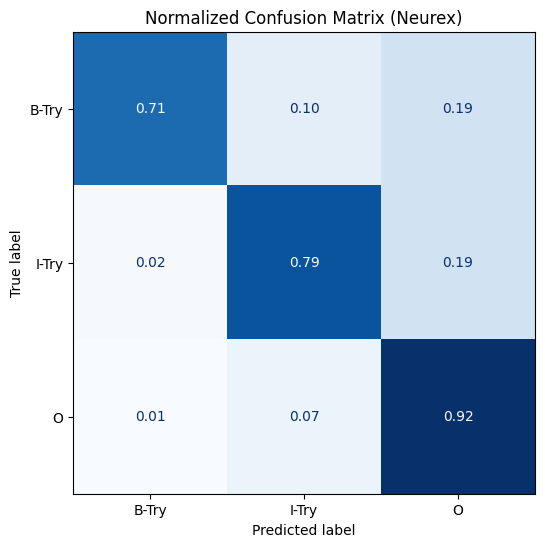
\includegraphics[width=2.4in]{rq2_cm_neurex.png}
        \vspace{-10pt}
 	\caption{Normalized Confusion Matrix --- {\tool} (XState Evaluated As Individual) (RQ2)}
 	\label{fig:rq2-cm-codebert}	
\end{figure}

\begin{figure}[t]
 	\centering
 	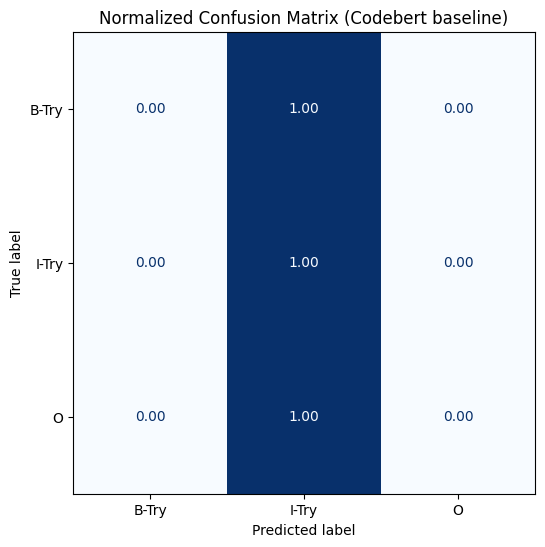
\includegraphics[width=2.4in]{rq2_cm_codebert.png}
        \vspace{-10pt}
 	\caption{Normalized Confusion Matrix --- CodeBERT baseline (XState Evaluated As Individual) (RQ2)}
 	\label{fig:rq2-cm-neurex}	
\end{figure}

%Table~\ref{tab:rq2} displays the result on detecting the statements
%that need to be placed in a \code{try-catch} block. $N_x$ is a parameter
%in GNNExplainer that defines the number of nodes in the explanation
%graph $\mathcal{G}_C$, i.e., the number of statements to be placed in the
%\code{try-catch} block.
%%
%As the number of nodes (statements) in $\mathcal{G}_C$ increases, the
%number of correct statements covered also increases, thus, accuracy
%increases. However, as the number of statements increases higher than
%5, accuracy increases more slowly. In our dataset, the average size of
%a \code{try-catch} block is 5.9 statements. As seen, the accuracy as
%$N_x$=6 is 74\%. That is, by pointing out 6 statements on average,
%{\tool} can correctly suggest 74\% of the total number of statements
%in the dataset that need to be placed in \code{try-catch}
%blocks. That is, it points out correctly 4.5 out of 6 statements to be
%in a \code{try-catch} block. For the statements that do not need to be
%placed in a \code{try-catch} block, {\tool} predicts correctly with
%63\% accuracy (not shown).
%
%\begin{figure}[t]
	\centering
	\lstset{
		numbers=left,
		numberstyle= \tiny,
		keywordstyle= \color{blue!70},
		commentstyle= \color{red!50!green!50!blue!50},
		frame=shadowbox,
		rulesepcolor= \color{red!20!green!20!blue!20} ,
		xleftmargin=1.5em,xrightmargin=0em, aboveskip=1em,
		framexleftmargin=1.5em,
                numbersep= 5pt,
		language=C,
    basicstyle=\scriptsize\ttfamily,
    numberstyle=\scriptsize\ttfamily,
    emphstyle=\bfseries,
                moredelim=**[is][\color{red}]{@}{@},
		escapeinside= {(*@}{@*)}
	}
\begin{lstlisting}[]
int ret = -1;
try {
  FileInputStream fin = new FileInputStream(path);
  int length = fin.available();
  byte[] buf = new byte[length];
  fin.read(buf);
  ret = loadFromBuffer(buf);
  fin.close();
} catch (FileNotFoundException e) {
    Log.e(TAG, "error:" + e);
    e.printStackTrace();
} catch (IOException e) {
    Log.e(TAG, "error:" + e);
    e.printStackTrace();
}
return ret;
\end{lstlisting}
        \vspace{-16pt}
        \caption{Correct Exception Handling Suggestion by {\tool}}
        \label{fig:example-experiment}
\end{figure}

%
%\vspace{2pt}
%\noindent {\bf Example.} Figure~\ref{fig:example-experiment} displays
%an example that {\tool} made correct suggestions. {\bf First}, it made
%a correct suggestion on the need of a \code{try-catch} block for the
%code at lines 1--8, 16.  {\bf Second}, GNNExplainer pointed out that
%{\xblock} used all the statements at lines 3--8 for such correct
%prediction. As a consequence, {\tool} correctly suggests to place
%lines 3--8 into a \code{try-catch} block. Note that, it also correctly
%pointed out that lines 1 and 16 do not need to be inside the
%\code{try-catch} block.  {\bf Third}, GNNExplainer gives three
%statements at lines 3, 6, and 8 highest scores. We can see that those
%lines contain three crucial API method calls: 1)
%\code{FileInputStream}, 2) \code{read}, and 3) \code{close}. {\bf
%  Fourth}, those three lines have data and control dependencies, which
%could help the model learn the identities of the API elements via
%their names \code{FileInputStream}, \code{read}, and \code{close},
%despite that the code snippet does not have the fully-qualified names
%for those API elements. This confirms the need of integrating {\em program
%  dependencies} in our solution. {\bf Finally}, {\tool} was also able
%to learn from the training corpus that those names refer to those API
%elements, which often correspond to the following exception types: 1)
%\code{FileInputStream} with \code{FileNotFoundException}, and 2)
%\code{FileInputStream.read} and \code{FileInputStream.close} with
%\code{IOException}.


%Note that {\tool} via {\xstate} predicts the statements to be placed
%in the \code{try-catch} block only after {\xblock} predicted that the
%given code needs such a block. Therefore, the incorrect cases from
%{\xblock} (i.e., those cases that need to be in a \code{try-catch}
%block but were predicted not) are also counted as incorrect in
%{\xstate}.

%{\color{red}{N1-N10 are the number of nodes that the subgraph contains which means the size of the try-catch block. Because the average size of the try-catch is 5.7, I currently pick 6 as the size of the try-catch block. The accuracy here is defined as: if a statement is in the try-catch block and our model put it in the subgraph, I regard it is correct $S_c$. All other conditions, I think they are incorrect. If there are $S$ statements in the try-catch block, the total accuracy is calculated as $S_c/S$. Later, I will add an example showing that the statement that our model predicted in the try-catch block contains the method call which lead to the correct exception types prediction.}}
